\documentclass[11pt]{article}
\usepackage[T1]{fontenc}
\usepackage[utf8]{inputenc}
\usepackage{lmodern,microtype}
\usepackage[margin=1in]{geometry}
\usepackage{amsmath,amssymb,amsthm,graphicx,booktabs,tabularx,array,longtable}
\usepackage[numbers,sort&compress]{natbib}
\usepackage{placeins}
\usepackage[colorlinks=true,allcolors=blue!40!black]{hyperref}
\usepackage{xcolor}
\hypersetup{pdftitle={How to design an assay that answers the biological question},pdfauthor={}}
\setlength{\emergencystretch}{2em}
\raggedbottom
\newcolumntype{Y}{>{\raggedright\arraybackslash}X}
\newcommand{\pos}[1]{[#1]_+}
\newcommand{\E}{\mathbb E}
\newcommand{\Prb}{\mathbb P}
\newtheorem{proposition}{Proposition}[section]
\title{How to design an assay that answers the biological question\\[5pt]
\large From specimen and signal to a justified biological conclusion}
\author{}
\date{}
\begin{document}
\maketitle
\begin{abstract}
An accurately measured signal can leave the biological question unresolved when sampling, population heterogeneity, stored material, or the measurement itself obscures the quantity of interest. This perspective examines how assay designers can identify competing explanations for a result and select observations or interventions that distinguish them. Three worked mathematical examples anchor the discussion. Pooled enzyme activity can conceal large differences in the fraction of units completing a recovery task; a calibrated functional readout narrows that range. Dilution can distinguish specified low and high analyte classes in a sandwich immunoassay, provided accessibility and measurement error are bounded. In microbial conversion, a two-pool material balance separates fresh entry from pre-existing inventory and explains why washing can strengthen inference even when less product is collected. Further examples examine specimen-level exclusion, recovery paths, preparation variability, stochastic amplification, and reporter sequestration. Drawing on assay validation, partial identification, and measurement-perturbation literature, we develop a workflow that starts with the intended claim and identifies the information needed to support it. The examples establish conditional mathematical results, with deterministic bounds and repeated-experiment error guarantees serving different reporting purposes. Their practical use requires validation of the relevant biological and measurement assumptions, including a rule for results that remain unresolved.
\end{abstract}
\noindent\textbf{Keywords:} assay design; biological function; partial identification; specimen recovery; measurement perturbation; formal verification.

\section{Start with the question the result must answer}
An enzyme preparation with the expected pooled activity may still contain many units unable to complete a particular task. Similarly, a low immunoassay signal may fail to establish low analyte concentration, and product collected during a microbial challenge may have been present before the challenge began. In each case, interpreting an accurately measured signal requires information about how it arose. Instrument calibration addresses only part of that problem: the specimen's history, heterogeneity, and route through the assay also determine which biological conclusions the result can support.

Assay developers already address many such issues through recovery controls, dilution studies, orthogonal measurements, reference materials, and validation in the intended matrix. The fit-for-purpose approach to biomarker measurement explicitly connects method development and validation to the intended use of the data \citep{lee}. Dilution linearity and hook-effect checks are established elements of ligand-binding bioanalysis \citep{ich}. Reporting guidance also places the intended use, reference standard, and handling of incomplete results at the center of interpretation \citep{stard}. The aim here is to make that connection inspectable: which alternative explanation does a control exclude, and which biological conclusion then follows?

Written for practicing assay designers and quantitative biologists, this perspective brings together eight mathematical case studies \citep{E,I,S,V,C,A,M,R}. Each specifies a biological target, an observation process, and a set of uncertainties. Some show how biologically different situations produce the same record; others establish what an additional observation or material balance can resolve. The main text develops their implications for design, with calculations in Appendix~\ref{app:derivations} and a proof-scope map in Appendix~\ref{app:map}. The underlying manuscripts are supplied as unpublished review material. All numerical examples are model constructions; applying their thresholds to an experimental or clinical setting would require validation.

The common design question is whether the explanations consistent with the observations agree closely enough to support the intended decision. For bounded measurement errors, this may require checking every compatible material history. For stochastic observations, it requires specifying the experiment and controlling the relevant error probability. We develop these approaches as tools for assay design, without treating their guarantees as interchangeable.

Partial identification provides a mathematical basis for this approach by describing what observations and assumptions determine when a unique answer is unavailable \citep{manski}. Set inversion similarly asks which inputs or parameters could have produced a bounded-error record \citep{jaulin}. Both allow useful conclusions without identifying every hidden parameter. The examples below apply this principle through population ranges, error-controlled reporting rules, and material balances.

\subsection{Name the target before choosing the readout}
Before choosing a readout, specify the quantity of interest and the conditions under which it is to be assessed. Measuring enzyme activity, for example, differs from estimating the fraction of units that reach a defined state by a deadline. Likewise, detecting no target in a well supports a claim about the original specimen only if sampling and recovery are accounted for. Defining the target at the outset prevents the interpretation from expanding beyond what the assay was designed to establish.

The denominator often determines whether a measurement answers the intended question. A fluorescence-weighted average may differ from a cell-number fraction, particularly when cells contribute unequal signals. Replication raises a related issue: two wells do not necessarily contain twice as much unique specimen, and ten images of one preparation do not provide ten independent observations of preparation variability. The analysis should therefore preserve both the unit to which the claim applies and the level at which observations are independent.

Table~\ref{tab:map} links each example to an experimental question. We develop enzyme recovery, sandwich immunoassays, and microbial conversion in detail, using the other cases to examine sampling, recovery, and measurement effects. Figure~\ref{fig:workflow} collects the resulting design questions into a workflow.

\begin{table}[t]
\centering\small
\caption{Experimental questions, competing explanations, and information that addresses them. Each row concerns a distinct model and its stated conditions.}\label{tab:map}
\begin{tabularx}{\linewidth}{@{}>{\raggedright\arraybackslash}p{0.17\linewidth}YY@{}}
\toprule Case & Biological question and obstruction & Information that changes the conclusion\\\midrule
Enzyme recovery \citep{E} & What fraction completes a task? Pooled activity hides the capacity distribution. & A functional-class readout with explicit calibration.\\
Immunoassay \citep{I} & Is native analyte low or high? Hooking and masking can both lower signal. & Dilution within a bounded model, plus native-availability evidence.\\
Specimen recovery \citep{S} & Can an original-specimen count be excluded? Sampling and shared failures intervene. & Unique specimen coverage and a native-reference reporting gate.\\
Recovery paths \citep{V} & Can a recoverable fraction be excluded? Available stages need not form a complete path. & Type-level path coverage, recording, and calibration guarantees.\\
Small populations \citep{C} & What count can be reached? Shared preparation changes multi-founder tails. & Calibration at the relevant preparation and observation level.\\
Amplification \citep{A} & Can loaded and blank reactions be separated? Their full timing laws overlap. & Identity-sensitive observation or changes to effective capacity.\\
Microbial conversion \citep{M} & Must output include fresh entry? Old mobile and reserve material can explain it. & A two-window material account and calibrated retention.\\
Reporter loading \citep{R} & Can a readout preserve function? The reporter stores a shared cofactor. & Residence-time, signal, and recovery budgets together.\\\bottomrule
\end{tabularx}
\end{table}

\section{The same average can support different functional populations}
\subsection{A precise pooled assay can leave the answer open}
Consider 82 equally weighted units. In one population every unit has catalytic capacity one. In another, 42 units have about 64.3\% of that reference capacity and 40 have 137.5\%. Their exact capacities give both populations mean capacity one (Appendix~\ref{app:enzyme}). A pooled measurement that adds capacity multiplied by the same response function therefore returns the same answer for both populations, at every admitted clamped initial-rate condition. Collecting a more precise version of that same pooled response does not reveal how capacity is distributed.

The functional question is different: what fraction reaches a specified carrier state by a deadline? The enzyme recovery model fixes a scalar rate law and lets catalytic capacity vary \citep{E}. Under its dynamics, all 82 units in the uniform population reach the target, whereas only the 40 high-capacity units in the heterogeneous population do. The target, initial state, and deadline are given in model units in Appendix~\ref{app:enzyme}. The two populations are observationally identical for the specified pooled assays and functionally different for the specified recovery task.

Cell-resolved G6PD assays provide an experimental example of measuring a distribution that aggregate enzyme activity can conceal \citep{shah}. Connecting such a readout to the recovery task considered here would require separate calibration of the dynamical endpoint. The present model describes that scalar task; it does not establish erythrocyte survival or patient risk.

The population bound goes beyond a pair of examples. Suppose capacities lie in two separated bands: roughly 62.5--64.3\% or 100--137.5\% of the reference capacity, with mean one and the fixed task dynamics. The exact compatible recovery range is approximately 48.78--100\%; the unrounded endpoints and support bands appear in Appendix~\ref{app:enzyme}. Every value in that interval is attainable by an admitted weighted population. Thus a claim that at least two-thirds recover is unresolved by the pooled record.

The separated capacity bands constrain how much low-capacity material can coexist with the high-capacity material needed to keep the mean at one. If capacities can instead accumulate just below the recovery threshold, the conclusion weakens substantially: in the companion's connected-support alternative, the lower endpoint becomes an unattained infimum of about 11.64\%. The population support is therefore a consequential assumption that requires evidence beyond the pooled mean.

\subsection{Add information about the unresolved variation}
Now add a readout calibrated to distinguish units that complete this task. Let $p$ be the recovery fraction, $s$ the sensitivity to that functional class, $f$ the false-positive probability, and $r$ the measured positive fraction. Their relation is
\begin{equation}\label{eq:readout}
r=sp+f(1-p).
\end{equation}
Suppose sensitivity is between 90\% and 100\%, the false-positive rate between 0\% and 2\%, and the observed positive fraction between 68\% and 72\%. Equation~\eqref{eq:readout}, together with the population constraints, narrows the exact compatible recovery range to approximately 67.35--80\%. Figure~\ref{fig:enzyme} shows the change. The unrounded lower endpoint exceeds two-thirds, so the designed requirement is supported.

The additional readout narrows the range by excluding populations inconsistent with its calibration and observed positive fraction, including the original 40-of-82 population. This is an identified set under bounded assumptions. If the positive fraction is estimated from a sample, a suitable simultaneous uncertainty statement must be incorporated before applying the bounds.

\begin{figure}[t]
\centering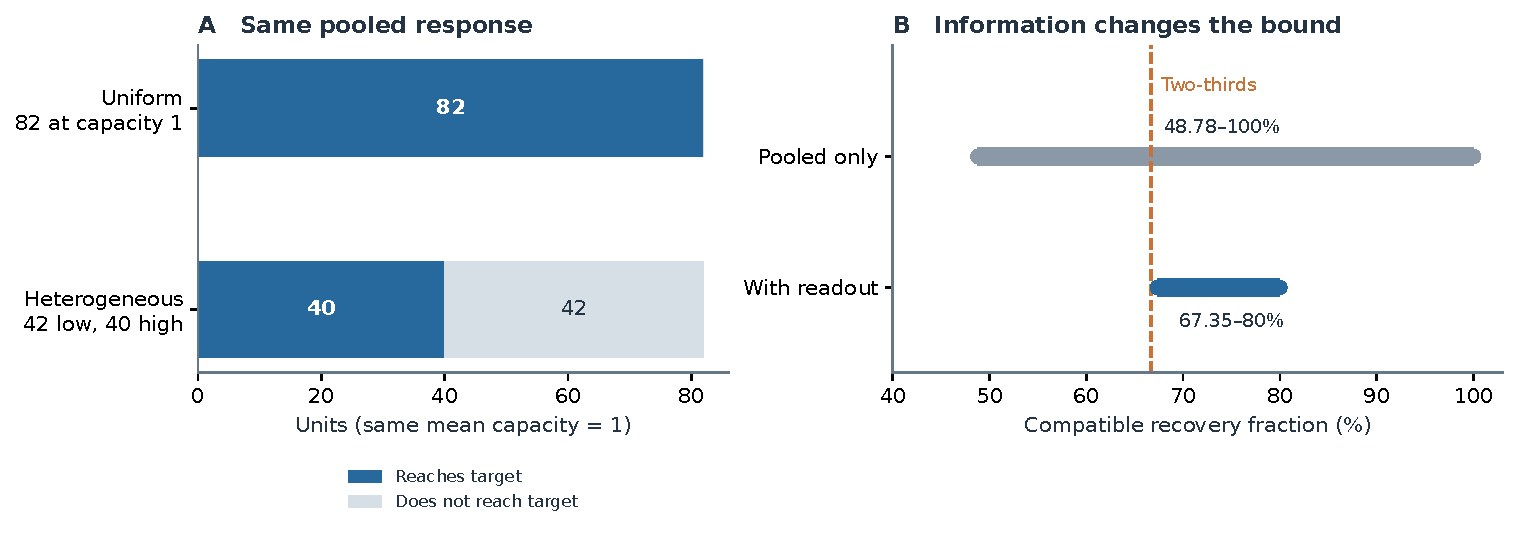
\includegraphics[width=\linewidth]{figures/enzyme.pdf}
\caption{Equal pooled activity, different task completion. Left: two 82-unit populations have the same mean capacity but 82 and 40 units, respectively, reach the source's target. Right: the exact compatible recovery interval under the separated-support model narrows after adding a calibrated functional readout. The dashed line is the designed two-thirds requirement.}\label{fig:enzyme}
\end{figure}

A useful second assay must constrain variation relevant to the recovery task. Another technology, even a nonlinear one, may still depend on the same population average and add no information about that variation. Conversely, a simpler aggregate feature may suffice without resolving individual cells. Appendix~\ref{app:enzyme} gives a linear-algebra test for exact identification over a finite population class and explains how useful bounds can remain available when exact identification fails.

Two implementation questions remain. First, are units weighted consistently? A readout dominated by cell size or enzyme abundance estimates a weighted fraction unless a justified normalization converts it to a number fraction. Second, does calibration represent units near the functional boundary as well as obvious positives and negatives? The decision margin here is small: the lower bound exceeds two-thirds by about 0.68 percentage points. Weighting error, off-support units, and calibration uncertainty must fit within that margin if this particular decision is to survive.

\section{A low signal needs a mechanism-specific explanation}
\subsection{Dilution can distinguish scarcity from excess}
A sandwich immunoassay records analyte bound to both capture and detection reagents. At low accessible analyte concentration, few sandwiches can form. At very high concentration, finite reagent supplies can occupy different analyte molecules, again leaving few sandwiches. This high-dose hook mechanism and dilution-based remedies have a long experimental history \citep{fernando,ich}. The mathematical example asks what a particular neat/diluted comparison certifies when reagent properties and measurements are uncertain \citep{I}.

The model distinguishes native concentration $x$ from accessible concentration $u=\rho x$, where $\rho$ is the accessible fraction. It assumes independent binding sites at equilibrium. Capture and detector capacities are $C,D$ and their dissociation constants are $K,J$. The sandwich concentration $B(u)$ follows reagent mass balances, not a fitted monotone response curve. Figure~\ref{fig:hook} plots this source at unit capacities and affinities. In this symmetric case, concentrations related by $u\mapsto4/u$ give identical neat signals, yet their tenfold-diluted signals differ.

The protocol dilutes the specimen before adding fresh reagents, so final reagent concentrations are preserved. Diluting a completed reaction would also dilute its reagents and would require a different calculation.

The uncertainty example admits all four reagent parameters in $[0.9,1.1]$, a dilution factor in $[9,11]$, and relative gain between readings in $[0.95,1.05]$. Over this entire box, the diluted-minus-neat source contrast is nonpositive for $u\le0.4$ and at least 0.04 for $20\le u\le100$. If native availability also satisfies $\rho\in[0.8,1]$, the native low class $x\le0.4$ and native high class $25\le x\le100$ inherit the separation.

\begin{figure}[t]
\centering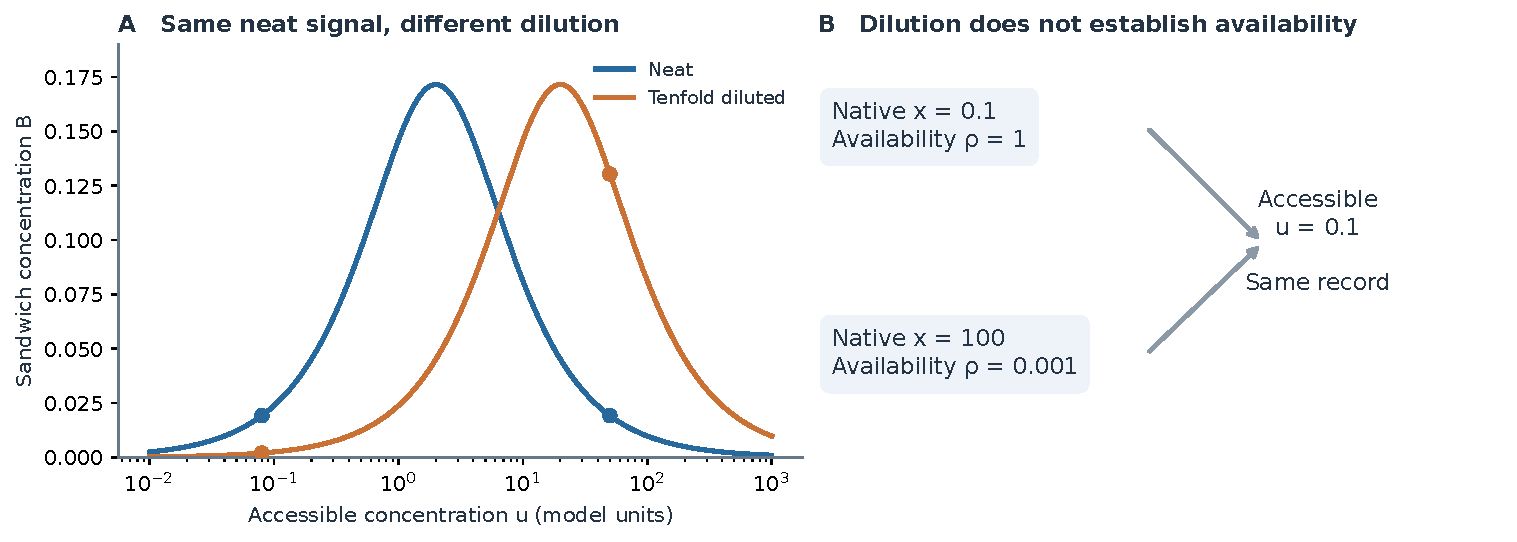
\includegraphics[width=\linewidth]{figures/hook.pdf}
\caption{Why dilution helps, and why it does not measure native availability. Left: the finite-reagent equilibrium source with $C=D=K=J=1$; the neat readings at $u=0.08$ and $u=50$ agree, while tenfold dilution separates them. Curves are floating-point illustrations of the mass-balance source. Right: native states $(x,\rho)=(0.1,1)$ and $(100,0.001)$ have the same accessible amount. Under the source's masking model, accessible spikes and dilution preserve this ambiguity. The severe-masking state lies outside the availability premise of the positive certificate.}\label{fig:hook}
\end{figure}

To separate the two classes, the gap between their predicted contrasts must exceed the measurement uncertainty on both sides. If each reading has absolute error at most $\varepsilon$ and common gain is at least one, strict separation requires $\varepsilon<0.01$ (Appendix~\ref{app:hook}). This requires an absolute error bound, which a coefficient of variation alone does not provide. A shared offset cancels across the pair, whereas separately varying offsets must be included in the allowance.

The contrast yields a binary decision only when the specimen is known to belong to one of the two stated concentration classes. Otherwise, a high contrast can exclude the low class, and a sufficiently low contrast can exclude the stated high class, while intermediate concentrations remain possible. Inverting the model over the full concentration domain can retain these intermediate or disconnected possibilities.

\subsection{A successful spike tests the route taken by the spike}
The masking example in Figure~\ref{fig:hook} shows why spike recovery cannot by itself establish native accessibility. A native concentration of 0.1 with full accessibility and a concentration of 100 with accessibility 0.001 both present accessible concentration 0.1. Adding a fully accessible soluble spike and applying dilution therefore produces the same records in the two model states. Successful recovery confirms that the added material can be measured, but leaves the native material's accessibility undetermined.

The dilution certificate assumes availability of at least 0.8, which excludes the high-native, low-accessibility state. Applying that certificate consequently requires independent evidence for availability. A native reference introduced before masking or extraction may help if its material form and interactions with the specimen allow it to follow the relevant processes. Its point of introduction determines which losses it can reveal.

The same reasoning limits the high-concentration tail. For any finite panel of bounded dilution factors, sandwich signals eventually approach blank-like values as analyte becomes arbitrarily large. With nonzero observation error, the panel cannot exclude every unbounded high concentration. A validated upper range changes this question; a numerical search cutoff does not. Sequential washing can alter the source, but fixed nonzero carryover can restore a high-dose tail. The relevant engineering question is therefore a finite-range carryover specification, not whether washing is universally protective against hooking.

\section{Interpreting negative results at the specimen level}
\subsection{Accounting for shared preparation failure}
Suppose the question concerns the number of native target units in the original well-mixed specimen. Two preparations examine distinct fractions of that material. In the specimen recovery model, the chance of a target being recovered depends on a state shared by all targets in its preparation \citep{S}. Conditional on those states, target paths are independent. The calculation therefore first determines the negative probability for each preparation state, then averages across states (Appendix~\ref{app:specimen}).

Averaging recovery before calculating the negative probability can substantially understate common failure. Suppose a preparation fails completely 5\% of the time and otherwise detects every target reaching it. Even many targets then leave a 5\% probability of a negative result. Assigning each target an independent 5\% failure probability would incorrectly make this probability decrease with target number.

A reporting rule can address this uncertainty using paired native references introduced before the relevant recovery steps. Each pair passes if at least one of its two native inputs is recovered. The rule issues an exclusion only when every reference pair passes and the future specimen is negative. The pairs and future specimen have independent states drawn from the specified common recovery population. Thus the references represent the distribution of preparation quality, rather than proving that the future specimen has a particular unobserved state.

In a balanced design examining two distinct 45\% fractions of the original specimen, nine reference pairs allow the rule to exclude six or more native units with worst-case false-issuance probability about 4.988\%. The experiment uses 18 native reference inputs and 18 reference preparations/readouts, plus two target-specimen preparations. The reference inputs are external to the target specimen. Under an illustrative law with independent 80\% recovery in each reference preparation, the gate passes about 69.25\% of the time; this is the certificate availability for a blank specimen under that law. Availability for a nonblank specimen also depends on its chance of testing negative. Appendix~\ref{app:specimen} gives the exact calculation.

More precisely, the guarantee concerns the following joint event:
\begin{quote}
Across the full reporting experiment, the chance of passing the reference gate and receiving a negative specimen result is at most the stated bound whenever the original specimen contains at least six native target units and the admitted recovery assumptions hold.
\end{quote}
It is not a 95\% posterior probability that this particular specimen has fewer than six targets. Nor does it bound the negative probability conditional on the gate having passed. The reported conclusion concerns fewer than six native units, not zero units, absence of organisms, or absence of disease. Appendix~\ref{app:specimen} displays the joint-event calculation and why conditioning would change it.

The resource comparison depends on how much unique material is sampled and what each replicate adds about recovery. Repeated observations of the same material cannot eliminate the chance that a target was never sampled. The worked design also leaves little room below 5\% for reference false positives or calibration error, and reusing a gate across a batch requires a corresponding batch-level analysis. Because a rule that rarely reports can have a low false-issuance probability, reporting availability should be evaluated alongside error.

\subsection{A recoverable unit needs a complete observed path}
Another negative assay asks whether a specified fraction of eligible units could complete a reference recovery task. This definition must be independent of whether the particular assay happens to observe them. In the paired-recovery model, each of two alternative conditions requires an activation stage followed by a progeny or qualifying-event stage \citep{V}. A complete path needs both stages in the same condition. Its probability is the chance of activation multiplied by the chance of completing the later stage given activation; this does not assume independence between stages.

For example, activation might always occur in the first condition while the later stage always fails; in the second condition, the later stage may be possible but activation may never occur. Neither condition then provides a complete path, however often it is repeated. Pooled stage averages can conceal this mismatch and leave a recoverable type unobserved.

The positive result bounds how well the two conditions cover each stage for each recoverable type, and how badly the stages can be mismatched within a condition. It then gives a minimum average probability of completing a path. Strong coverage can force a positive minimum even with loose mismatch information: when the two conditions' probabilities sum to more than one at each stage, their overlap cannot be eliminated entirely. Appendix~\ref{app:paths} gives the sharp result over the full coverage range, including coverage levels that yield detection floors above 25\%.

The design must also allow for recoverable types outside the calibrated coverage and for completed events that fail to be recorded. After those allowances, a positive detection floor determines how many independent eligible units are needed to bound an all-negative result. A calibration-failure allowance requires the future-experiment bound to hold conditional on valid calibration; a marginal calibration confidence statement alone does not provide that guarantee.

In practice, calibrating a detection floor directly on representative, independently established reference-positive units may be simpler than estimating every stage separately. The reference task must include its follow-up period, since timing data from observed successes give no direct estimate of units that leave no record. Bacterial persistence provides a related reason to define endpoints carefully: surviving cells can regrow while retaining antibiotic sensitivity, so recovery and resistance have different biological meanings \citep{balaban}.

\section{Choose observations that address the actual uncertainty}
\subsection{Preparation can change the prediction from identical founder evidence}
Single-founder growth records may not determine a multi-founder prediction. The small-population example compares latent growth classes assigned independently to founders with a class shared by all founders in one well \citep{C}. The complete chronological observation law for one founder is identical in the two preparations. At the model's specified horizon, however, the minimal 95\% upper count cutoff for two founders is six under independent classes and seven under the shared class. The probabilities of being at or below six are about 95.70\% and 94.53\%, respectively. Appendix~\ref{app:counts} supplies the horizon, preparation laws, and exact probabilities.

A shared preparation state changes the joint behavior of founders even when their individual growth laws are unchanged. Repeated imaging of one well can characterize its trajectory, but estimating preparation variation requires independent wells. The latent growth classes in this example describe the mathematical source; assigning them a mechanism such as antimicrobial resistance would require further evidence.

A cutoff of seven is valid for both preparations, so calibration is useful when the narrower cutoff of six matters to the application. Under a particular exact-binomial procedure, the source compares sufficient designs requiring 1,280 and 640 independent calibration wells. These costs motivate choosing a statistic that separates the relevant preparation laws efficiently; they do not establish an optimal design.

A detector can change that answer. With independent thinning, the difference between the two preparations in the probability of recording at most two cells vanishes at detection probability one-half and reverses below it. That statistic has lost its discriminatory value at one-half; the full observed law has not necessarily become identical. Another statistic can still separate the models. This distinction prevents an uninformative summary from being mistaken for a proof that all available data are uninformative.

Detection loss also changes the endpoint being bounded. Missing cells may make a bound on the recorded count easier to satisfy without supporting the same bound on the biological count. We use the exact preparation model here; the companion's limited empirical audit, with unresolved outcomes and a single held-out run, provides insufficient evidence to establish general predictive coverage.

\subsection{When timing information is insufficient}
Digital PCR separates template molecules into reactions and uses product identity to count classes of molecules \citep{vogelstein}. The amplification model considered here examines what can be inferred from threshold-crossing time alone \citep{A}. It includes spontaneous initiation, growth, finite capacity, and a latched crossing time. A reaction assigned to the target-loaded condition can still contain no target after Poisson loading; such reactions remain in the denominator when evaluating missed detections.

At spontaneous-to-growth rate ratio $b/g=0.01$, mean loading four, and threshold equal to capacity five, the source proves that every randomized measurable classifier using the complete crossing time has miss probability greater than 5.55\% if blank false positives are at most 1\%. This rules out more than a poorly chosen deadline: even unrestricted use of that timing observation cannot achieve the stated pair of errors. A conventional optimal-deadline argument supplies a stronger bound in its fixed-rate setting, but the simpler all-classifier statement suffices for the present design lesson.

Adding a constructed hit-plus-identity observation at time seven reduces blank error below 0.03\% and miss probability below 4.23\% under the model's conditional marker assumptions. Experimental implementation would require a marker satisfying those error bounds while preserving the relevant kinetics. The reporter model in the next section illustrates why this second requirement can be demanding.

Several interventions can therefore improve an amplification assay, but they act on different constraints. Adjusting the deadline changes how existing timing information is used, whereas recording identity adds an observation and increasing effective capacity changes the reaction dynamics. The companion's large-threshold capacity results concern a different regime from the five-state example, so their practical implications depend on the relevant kinetic model.

Poisson loading imposes a separate limit: the empty fraction alone gives a miss floor $e^{-\lambda}(1-\alpha)$ under blank-error allowance $\alpha$. At $\lambda=4$ and $\alpha=0.01$, this is about 1.813\%. Partitioning a fixed stock across more wells changes the loading distribution while preserving the finite supply of target molecules. The analysis must also retain noncrossers and account for incomplete records. If the decision time is selected after inspecting the data, the uncertainty statement must cover that selection; otherwise the rule should be fixed in advance. These requirements complement established guidance on amplification controls and raw-data reporting \citep{miqe}.

\section{Account for what was already there and what the test changes}
\subsection{Fresh conversion is a material-history question}
A microbial preparation yields product during a challenge. Some product may have been generated during the observation period; some may have been extracellular at the start; some may have been stored in a reserve and released later. A functional conclusion requires a boundary around the material being credited. The microbial material-balance model uses two pools, mobile product and convertible reserve, with two collection windows separated by a recovery or wash step \citep{M}.

The reserve must include any pre-existing source that could contribute product-equivalent material, such as relevant biomass, sorbed material, or convertible intermediates, with conservative bounds on conversion yield. An omitted source would otherwise be counted as fresh production. All amounts refer to the original aliquot, and each collection is credited once; endpoint concentrations and wash waste require explicit conversion to the defined collected amount.

In this accounting, ``fresh'' means entry into the declared credited inventory during the windows. It does not by itself establish substrate-specific atom provenance, gross synthesis of a particular molecule, viability, restoration of previous function, or future productive capacity. Isotopic tracing and dynamic metabolic flux analysis address related attribution questions with their own observation models \citep{leighty}. Which substrates are supplied also defines which pathway is challenged. Established cross-feeding experiments illustrate that pathway relationships can depend on the organisms and substrates involved \citep{belenguer}; feeding downstream of a community member cannot alone demonstrate that member's upstream contribution.

The calculation can be explained without fitting every uptake and release rate. First ask how much of the early collection could have come from the initial stock. Then ask how much old material could remain after that collection and survive the intervention. Finally add any credited material introduced during recovery. A later collection exceeding that allowance forces fresh entry somewhere in the two windows.

Combining lower bounds on collection with upper bounds on initial inventory, pre-wash reserve, and recovery inputs gives the least fresh entry consistent with the retained fractions of both pools. This bound is sharp over the stated material histories because an admitted schedule attains it (Appendix~\ref{app:material}). Strain-specific kinetic constraints may rule out that schedule and strengthen the bound.

\subsection{Less collected product can give stronger evidence of fresh entry}
Consider the synthetic matched example in Figure~\ref{fig:material}. Initial inventory is bounded by 10, pre-wash reserve by 2, and recovery input by 0.2 in product-equivalent units. The first reading is 6 with error allowance 0.2, so at least 5.8 was collected. In the washed branch, 5\% of mobile material and 90\% of reserve can be retained, and the second reading is 4 with error allowance 0.2. The material account forces fresh entry of at least 1.69.

In the physically matched unwashed branch, both retention factors are 90\%, and the second reading rises to 5.7. Its fresh-entry lower bound is 1.52. Both branches have an admitted history with fresh amount 2.1. The wash changes carryover and therefore changes the record. Holding the second record artificially fixed while comparing retention factors would give the intervention credit for a comparison it did not produce.

\begin{figure}[t]
\centering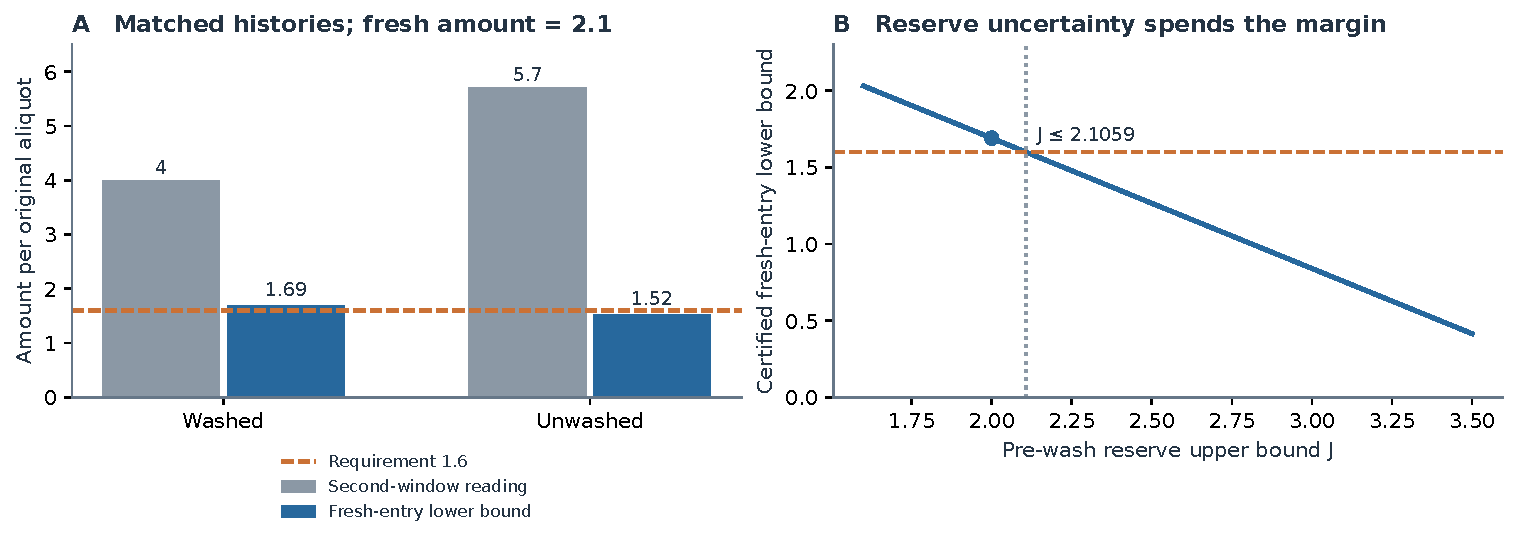
\includegraphics[width=\linewidth]{figures/material.pdf}
\caption{A matched wash comparison. Both constructed histories have fresh amount 2.1. The washed branch collects less in the second window but yields a stronger lower bound, 1.69 versus 1.52, because less of the record can be explained by retained old material. The designed requirement 1.6 is supported only by the washed record. Right: sensitivity to the pre-wash reserve allowance in this worked family; the washed bound reaches 1.6 at a reserve allowance of approximately 2.106. Quantities are product-equivalent units per original aliquot.}\label{fig:material}
\end{figure}

The intuition is that the second collection carries two messages at once: some material may be fresh, and some may simply have carried over. Without washing, uncertainty about the old mobile stock survives into the second window and can explain more of its output. Washing removes most of that mobile contribution. The collected amount falls, but the allowance that must be reserved for old material falls enough to strengthen the lower bound on fresh entry. If the old stock were known exactly, merely removing it would not supply this uncertainty-reduction benefit. The gain here comes from making an uncertain alternative explanation smaller.

At a requirement of 1.6, the washed record supports the claim while the unwashed record leaves it unresolved. The gain is modest, however, and uncertain reserves or loss of biological activity can erase it. The companion derives a break-even activity condition for this matched family, separating retention of material from retention of function.

The timing of the reserve bound is decisive. Initial reserve two does not imply pre-wash reserve at most two: uptake during the first window can move mobile material into the better-retained pool. The companion constructs a zero-fresh history that receives a false positive lower certificate if the initial bound is substituted for the later one. Direct reserve measurement is one remedy. Another proved remedy combines an initial reserve bound with a bound on cumulative gross uptake. Net extracellular disappearance does not automatically bound gross uptake, because release and reuptake can occur in the same window.

Reporting the lower bound together with the inventory assumptions and collection windows makes the conclusion interpretable. A bound below the required amount leaves the claim unresolved; excluding it requires an upper bound. Conflicting bounds instead call for investigation of the model or calibration. A killed or no-substrate control can inform this analysis if its material balance is sufficiently well matched to that of the live challenged preparation.

\subsection{A reporter can store the resource it is meant to observe}
Measurement can change the hidden history as well as reveal it. The reporter-loading model retains an explicit complex between a reporter and a shared cofactor \citep{R}. A reduced cofactor supports a target reaction and is regenerated from its oxidized form. When the reporter binds the reduced cofactor, it temporarily removes that material from both target use and regeneration. A model that replaces the reporter by instantaneous consumption deletes this storage compartment.

The biological importance of downstream loading and resource competition is established in the literature on retroactivity: connecting a downstream process can alter the upstream process that drives it \citep{delvecchio}. Here the explicit cofactor model permits an exact cost account. For matched preparations and finite total association exposure, the loss of target output per reporter product depends on how long successful turnover stores cofactor. At regeneration coefficient one and catalytic release coefficient 0.2, the loss is six times the instantaneous-turnover prediction. Figure~\ref{fig:reporter} shows how faster release reduces this additional burden. Appendix~\ref{app:reporter} derives the identity and states the analytic assumptions needed for complete recovery.

\begin{figure}[t]
\centering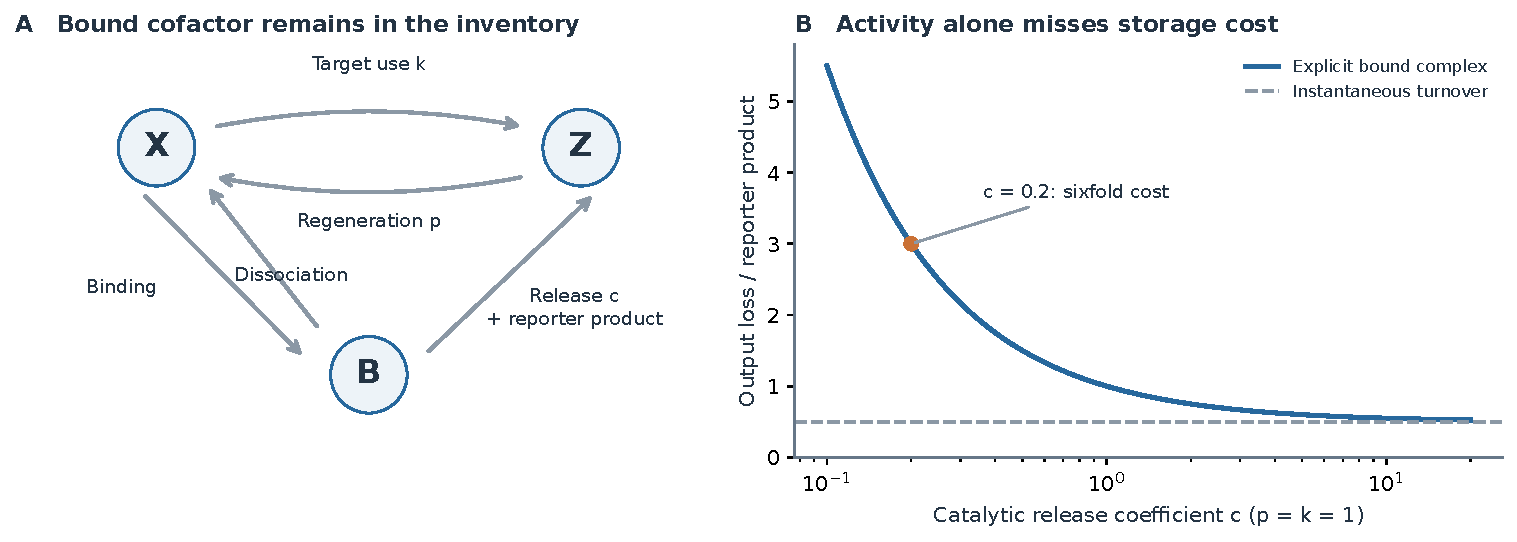
\includegraphics[width=\linewidth]{figures/reporter.pdf}
\caption{Reporter storage and the cost of information. Left: cofactor cycles between reduced $X$ and oxidized $Z$ forms, while reporter-bound $B$ temporarily removes material from both free pools. Catalytic release generates reporter product; dissociation returns reduced cofactor. Right: complete-recovery target-output loss per reporter product at $p=k=1$. The explicit-complex cost exceeds the instantaneous-turnover value 0.5 by a factor $1+1/c$. At $c=0.2$, it is 3.}\label{fig:reporter}
\end{figure}

Within this model, rescheduling acquisition leaves the complete-recovery cost unchanged at fixed final reporter product, although it can alter transient suppression and when information becomes available. Shortening exposure reduces total loss by producing less signal. Reducing the cost per product instead requires changing features such as resource supply or catalytic release, which alter cofactor residence time or the underlying balance.

The companion also identifies a parameter region in which an eight-unit acquisition separates two specified functional classes while target-flux suppression remains below 4.73\% throughout acquisition and recovery. This provides a worked example of jointly designing information gain and preservation within an explicit kinetic model.

Recovery continues after new association stops because existing complexes still contain cofactor. The source treats both an ideal switch and a fading association flux, in each case preserving the cofactor inventory. Removing reporter together with bound cofactor would change that balance. Evaluation must also distinguish the residual deficit after recovery from target output already lost during acquisition.

Target specificity remains a separate calibration problem. In the model, a hidden background consumer permits identical reporter trajectories with stationary target fluxes differing threefold. Measuring total consumption precisely therefore leaves the target's contribution unresolved unless independent information distinguishes the two consumers. Here the term ``native'' denotes the target channel in the constructed assay.

\section{Matching the report to the evidence}
The examples support different reporting statements because they address different uncertainties. The enzyme calculation gives an exact compatible population range, whereas the microbial balance gives a sharp lower bound over material histories. The specimen procedure controls false issuance over repeated experiments, and the growth calculation predicts a future count under a preparation law. Reports should name the relevant guarantee so that readers can interpret its scope.

For a deterministic threshold claim, a compatible lower bound above the threshold supports the claim, an upper bound below it refutes the claim, and an interval spanning it leaves the decision unresolved. This interpretation requires at least one feasible explanation of the record. If a calculation encloses all feasible values and returns an empty set, the record conflicts with the model or calibration assumptions. A nonempty enclosure, however, can contain unattainable values, so feasibility may require a separate witness; a solver's failure to find one does not establish incompatibility.

For stochastic observations, nonzero likelihood alone usually admits too many alternatives to guide a decision. The reporting guarantee must refer to a specified experiment and error criterion: a 5\% false-issuance bound, a 95\% prediction region, and a 95\% confidence procedure describe different repeated-experiment properties. Interpreting a result as the probability of a biological condition in one specimen requires additional assumptions. Clinical interpretation also depends on the intended population and the role of the test.

The reporting rule should specify how incomplete and inconclusive records are handled. Instrument failure may make a result unevaluable, a valid interval spanning the decision threshold leaves it unresolved, and a record inconsistent with every admitted model state indicates incompatibility. Excluding these outcomes from the denominator can inflate apparent performance. STARD's guidance on participant flow and indeterminate results is relevant when evaluating such procedures in diagnostic accuracy studies \citep{stard}.

Table~\ref{tab:report} pairs example conclusions with the assumptions needed to interpret them. In routine use, a laboratory could define this scope once and associate it with subsequent results, with an explicit procedure for exceptions.

\begin{table}[t]
\centering\small
\caption{Examples of supported statements and their required scope. All numerical thresholds refer to constructed source examples.}\label{tab:report}
\begin{tabularx}{\linewidth}{@{}YY@{}}
\toprule Statement & Scope that must accompany it\\\midrule
``At least two-thirds complete the task.'' & The scalar target and deadline, separated capacity support, consistent weighting, and calibrated positive-fraction bounds.\\
``The declared low native class is excluded.'' & The independent-site source, availability, concentration domain, dilution protocol, and simultaneous error allowance. Intermediate values may remain.\\
``The procedure excludes six or more native units.'' & Original-specimen coverage and reference gate; the bound concerns false issuance over the full experiment.\\
``Fresh credited entry is at least 1.69.'' & Two windows, original aliquot, full old inventory, pre-wash reserve, retention, and recovery-input bounds.\\
``The readout meets a preservation bound.'' & The explicit reporter source, matched baseline, parameter region, acquisition and recovery protocol; cumulative loss is reported separately.\\\bottomrule
\end{tabularx}
\end{table}

\section{Design backward from the intended decision}
Figure~\ref{fig:workflow} organizes these questions into a design process, from defining the claim to validating a rule for issuing it. The following application illustrates how the steps fit together.

\begin{figure}[tbp]
\centering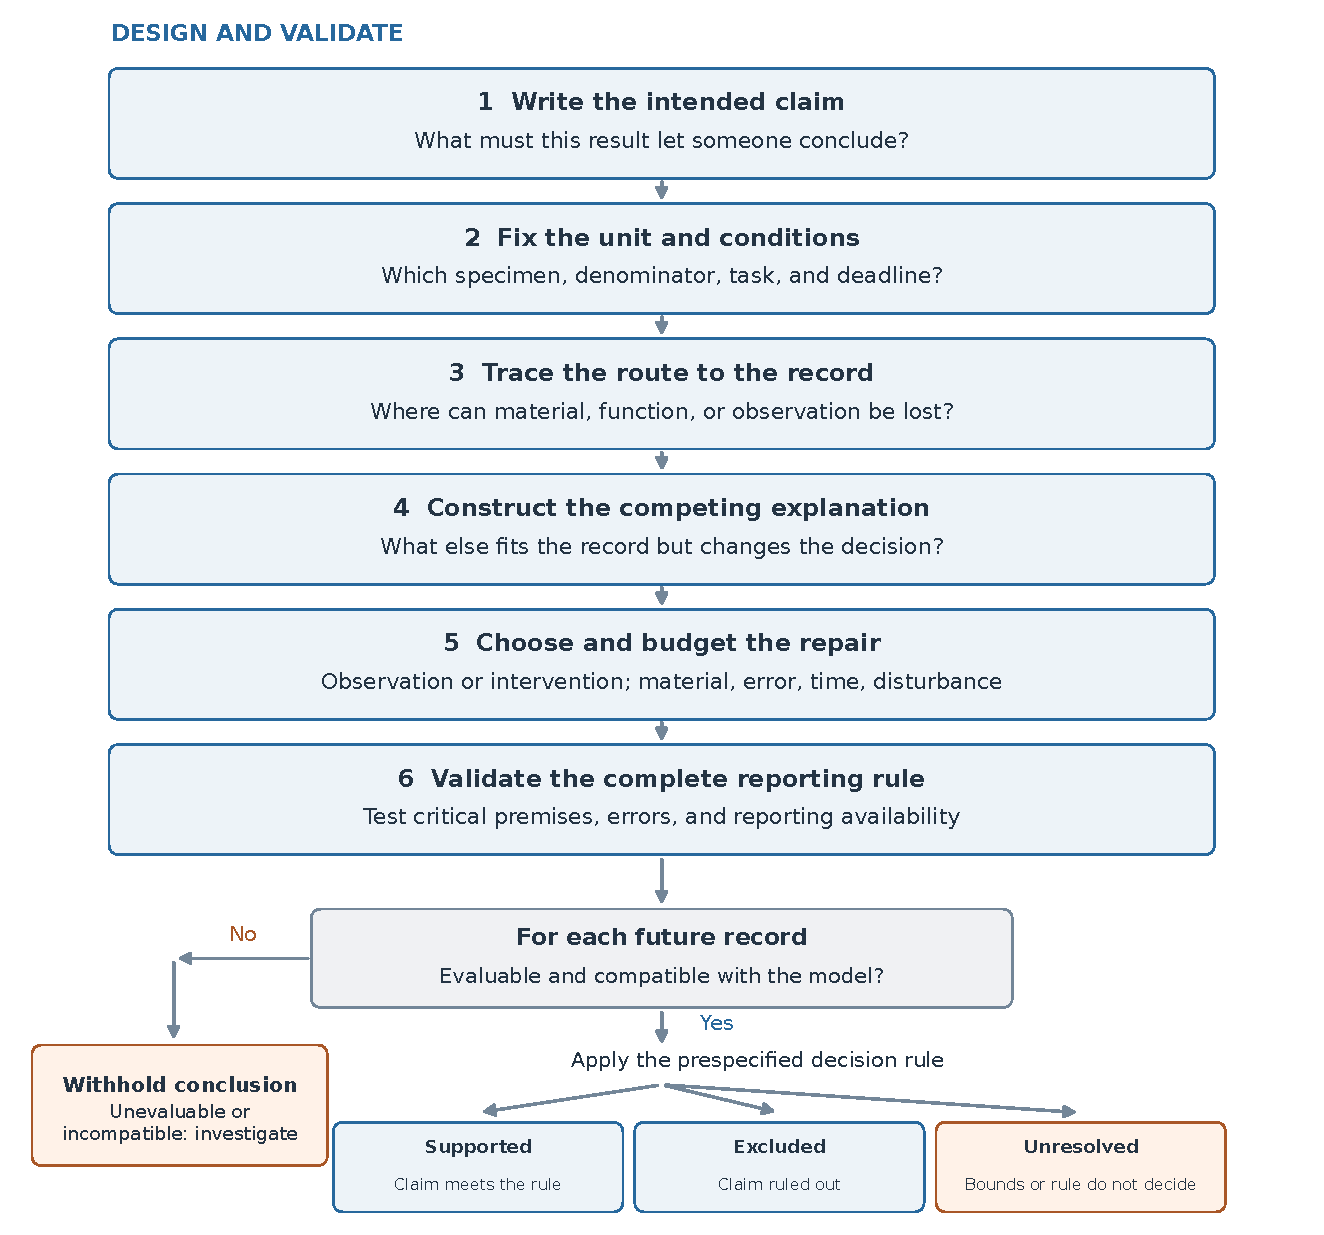
\includegraphics[width=\linewidth]{figures/workflow.pdf}
\caption{A workflow connecting the intended claim to a validated reporting procedure. The first five steps define a proposed reporting rule; the sixth evaluates the complete procedure before use. On a future record, compatibility and evaluability are checked before applying the prespecified rule. An unresolved result remains distinct from a missing record or a model-incompatible result. Statistical rules retain their stated error guarantee; the final branches do not turn that guarantee into a posterior probability.}\label{fig:workflow}
\end{figure}

Consider a researcher using the microbial challenge to establish fresh entry of at least 1.6 product-equivalent units per original aliquot. The claim fixes the target for step 1; specifying the two collection windows and aliquot defines step 2. Tracing old mobile and reserve material through the wash addresses step 3 and identifies carryover as the competing explanation in step 4. The matched comparison then evaluates a proposed intervention: washing lowers the second reading but raises the fresh-entry lower bound from 1.52 to 1.69, enough to support the claim under the stated assumptions (step 5). Before using that reporting rule, step 6 requires calibration of retention, recovery inputs, and especially the pre-wash reserve, together with an assessment of activity lost during washing. If the validated bounds span the requirement, the report remains unresolved.

Other assays follow the same sequence with different sources of ambiguity. A pooled enzyme measurement may need information about the capacity distribution, while an immunoassay may need evidence of native accessibility. Tracing the specimen through the procedure helps identify where a control should enter: a reference introduced after extraction can assess later losses but cannot estimate extraction loss without additional information. The useful control is the one that tests the alternative explanation affecting the intended decision.

The choice of intervention also depends on practical cost. A narrower prediction may require more independent preparations than the application can support; improved exclusion may come at the cost of rarely issuing a result. Similarly, washing can improve attribution while reducing useful biological activity. Comparing these trade-offs requires the same endpoint and, where possible, matched histories, so that apparent information gains are not produced by changing the question.

Validation should concentrate on assumptions whose uncertainty could change the decision. For the enzyme example, the small margin above two-thirds makes weighting and functional calibration especially consequential. For the microbial example, the timing of the reserve bound matters because material can move into reserve before washing. These analyses help prioritize the next experiment by showing which uncertainty most limits the conclusion.

The complete reporting procedure should then be evaluated prospectively in the intended setting, retaining unresolved and unevaluable outcomes. Separating development from performance evaluation allows the mathematical stress tests to guide, rather than substitute for, experimental assessment of matrix effects, drift, and preparation variability. The resulting assay is useful when its reported conclusion follows from both the measurement and the validated conditions under which that measurement was made.

\section*{Evidence, scope, and reproducibility}
The eight technical manuscripts underlying the worked models are included as accompanying review material and cited as unpublished manuscripts in the versions examined. No public archive identifiers were supplied. Appendix~\ref{app:derivations} gives selected derivations for the central examples; Appendix~\ref{app:map} identifies further source dependencies and distinguishes machine-checked implications from conventional proofs. The article reports no new biological experiments or clinical validation.

The source package includes editable \LaTeX, bibliographic records, figure-generation code, exact-arithmetic checks, and file provenance. Numerical curves illustrate the models; the accompanying derivations establish the stated bounds.

\FloatBarrier
\appendix
\section{Selected derivations and assumptions}\label{app:derivations}
\subsection{Population recovery and a calibrated readout}\label{app:enzyme}
The scalar recovery task starts at carrier state 10, targets state 28, and has deadline 120 in the model's units. Capacity lies in $[5/8,9/14]\cup[1,11/8]$ and has mean one. The exact compatible intervals are $[20/41,1]$ from pooled information and $[33/49,4/5]$ after the stated functional readout. Rounded percentages in the main text describe these intervals; calculations use the exact endpoints.

The two 82-unit populations have equal mean because
\[
42\frac9{14}+40\frac{11}{8}=27+55=82.
\]
In the source's separated support, all capacities in the lower band fail the task and all in the upper band complete it. If $p$ is the upper-band mass, its mean can be at most $(1-p)9/14+p\,11/8$. The mean-one constraint therefore gives $p\ge20/41$. The upper bound is one, attained by the uniform population. The kinetic classification, literal source solutions, and attainment of all intermediate fractions are proved in E; the mean calculation alone would not establish task completion.

For the calibrated readout, the largest positive fraction at given $p$ is $p+0.02(1-p)$ and the smallest is $0.9p$. Thus compatibility with $r\in[0.68,0.72]$ requires
\[
0.68\le0.02+0.98p,\qquad0.9p\le0.72,
\]
or $33/49\le p\le4/5$. For any $p$ in this interval the attainable readout interval $[0.9p,0.02+0.98p]$ intersects $[0.68,0.72]$, so suitable $s,f,r$ exist. E supplies a population witness in the same mean-constrained kinetic class. The decision margin is $33/49-2/3=1/147$.

For completeness, the general finite-feature principle behind this example has a short conventional proof \citep{E}. Let population weights $w$ range over a finite simplex, observations be $Aw$, and target be $b^\top w$. Include the normalization row $(1,\ldots,1)$ in $A$. The target is determined by the observations for \emph{every} population precisely when $b^\top$ belongs to the row span of $A$. Sufficiency follows by writing $b^\top=v^\top A$. If the condition fails, linear algebra provides $h\in\ker A$ with $b^\top h\ne0$. The normalization row gives $\sum h_i=0$. For an interior weight vector $w_0$ and sufficiently small $\epsilon>0$, both $w_0\pm\epsilon h$ are populations with the same observations and different targets. This global obstruction does not preclude exact identification at a particular boundary record, or a useful threshold bound without point identification. This argument is conventional; we do not represent it as a newly compiled Lean theorem.

\subsection{Dilution, physical occupancy, and the error budget}\label{app:hook}
Write the capture and detector occupation fractions as $p_C,p_D$. The independent-site equilibrium source satisfies
\[
C=up_C+\frac{Kp_C}{1-p_C},\quad
D=up_D+\frac{Jp_D}{1-p_D},\quad B(u)=up_Cp_D.
\]
For $C,K>0$, the physical root is
\[
p_C=\frac{2C}{u+C+K+\sqrt{(u-C)^2+2K(u+C)+K^2}}.
\]
The same formula with $D,J$ gives $p_D$. This is the formula used in Figure~\ref{fig:hook}; it satisfies the reagent balances and gives $B(u)\sim CD/u$ at high concentration. At unit parameters, $B(0.08)=B(50)$ by the source involution. The plotted equality is illustrative of the exact structure, not a numerical proof of it.

With observations $Y_1=gB(u)+e_1$ and $Y_d=grB(u/d)+e_d$, the contrast is $Z=g\Delta+e_d-e_1$. Let $|e_1|\le\varepsilon_1$, $|e_d|\le\varepsilon_d$, and $g\ge g_{\min}>0$. Source bounds $\Delta\le0$ on one class and $\Delta\ge m$ on the other imply
\[
Z\le\varepsilon_1+\varepsilon_d\quad\hbox{on the low class},\qquad
Z\ge g_{\min}m-\varepsilon_1-\varepsilon_d\quad\hbox{on the high class}.
\]
The two ranges are strictly separated when $2(\varepsilon_1+\varepsilon_d)<g_{\min}m$. Taking $g_{\min}=1$, $m=1/25$, and equal errors gives $\varepsilon<1/100$. Source I proves the continuum margin over $C,D,K,J\in[9/10,11/10]$, $d\in[9,11]$, and $r\in[19/20,21/20]$ by exact polynomial certificates. A plotted unit-parameter curve is not a substitute for those certificates. The availability model treats the inaccessible fraction as invisible to both sites; partially masked material that consumes one reagent requires a different source model.

\subsection{A joint reporting event, not a posterior}\label{app:specimen}
Let $N$ be the original-specimen target count, $a,b$ the unique effective fractions examined, and $X,Y$ the two state-dependent recovery probabilities, with $a+b\le1$. Conditional independence of target paths gives negative probability $\E[(1-aX-bY)^N]$. The preparation-state average is taken after the power because the state is shared; replacing $X,Y$ with their means generally does not preserve this probability.

For balanced unique effective fractions $a=b$, count threshold $K$, and $m\ge1$ independent reference pairs, set $H=(1-a)^K$. Study S reduces the sharp false-issuance bound to
\[
G_m(H)=\max_{0\le z\le1}z^m\{1-(1-H)z\}.
\]
The reduction uses the full recovery-law optimization and the paired-reference experiment; it is not obtained merely by guessing a scalar recovery probability. Differentiating the final polynomial gives
\[
G_m(H)=
\begin{cases}
H,&H\ge1/(m+1),\\[2pt]
\displaystyle\frac{m^m}{(m+1)^{m+1}(1-H)^m},&H<1/(m+1).
\end{cases}
\]
At $a=9/20$, $K=6$, $m=9$, $H=(11/20)^6=0.027680640625$ and $G_9(H)\approx0.0498772$. The exact rational value is reproduced in the calculation file. The limiting floor $H$ has a material origin: even favorable recovery cannot find a target in an unexamined part of a specimen.

Let $G$ denote gate passage and $N_-$ the negative record. The theorem bounds $\Prb(G\cap N_-)$ for each admitted law when the target count is at least $K$. In contrast, $\Prb(N_-\mid G)=\Prb(G\cap N_-)/\Prb(G)$, when the denominator is positive. A joint bound alone does not give the same conditional bound. A posterior probability of count below $K$ would additionally require a prior and a likelihood model. These distinctions do not diminish the usefulness of the reporting rule; they specify the experiment for which its reliability is proved.

\subsection{Complete paths across the full coverage range}\label{app:paths}
The uniform type-level conditions in V are $0\le x,y,a,b\le1$, $x+a\ge c$, $y+b\ge c$, and $|x-y|\le d$, with $0\le c\le2$ and $d\ge0$. Here $x,y$ are the successive stage probabilities in the first condition, and $a,b$ those in the second. The exact balanced floor is
\[
R(c,d)=\frac{c^2-t^2}{4},\qquad t=\min\{d,c,2-c\}.
\]
To see the geometry, first reduce the cross-condition sums to $c$ by clipping the first-condition probabilities into $[\max(0,c-1),\min(c,1)]$. This can only reduce the complete-path lower expression and cannot increase the distance between the clipped values $X,Y$. The remaining algebra is
\[
\frac{XY+(c-X)(c-Y)}2
=\frac{c^2-(X-Y)^2+(X+Y-c)^2}{4}\ge R(c,d).
\]
Taking $X=(c+t)/2$, $Y=(c-t)/2$, $a=Y$, $b=X$ attains the bound. The choices lie in $[0,1]$ because $t\le c$ and $t\le2-c$. In particular, for $c>1$, $R(c,d)\ge c-1$.

With recorded mean path probabilities $u,v$ satisfying $(u+v)/2\ge g$, recoverable fraction $p\ge\theta$, and $n=2m$ independent units split equally, the all-negative probability is $(1-pu)^m(1-pv)^m\le(1-\theta g)^n$. If this holds in every valid calibration environment and invalid environments have probability at most $\delta$, the full bound is $\delta+(1-\delta)(1-\theta g)^n$. Validity conditional on the calibration environment is essential. V also proves a mean-square mismatch extension; it should not be confused with a bound inferred from pooled stage averages alone.

\subsection{The two-founder calculation and the loading floor}\label{app:counts}
At $T=\log2$, a fast Yule family has $\Prb(Z=j)=2^{-j}$ for $j\ge1$, while a slow family stays at one. Each founder's marginal class is half slow and half fast. Independent classes give mixture weights $1/4,1/2,1/4$ for two slow, mixed, and two fast families; the shared class gives weights $1/2,0,1/2$. Hence, for $k\ge2$,
\[
F_I(k)=1-\frac{k+5}{4\,2^k},\qquad
F_W(k)=1-\frac{k+1}{2^{k+1}}.
\]
At $k=6$, these are $245/256$ and $121/128$; at $k=7$, $125/128$ and $31/32$. A single chronological family record has the same mixture law in both preparations. The difference enters only when multiple founders are combined. C's formal development verifies the relevant chronological source calculation and finite cutoffs; the general formula is also derived conventionally in that manuscript.

For the separate amplification model A, let $M$ be a Poisson-loaded initial target count with mean $\lambda$. Conditional on $M=0$, its observation law is the blank law. Any classifier with blank false-positive probability at most $\alpha$ therefore has miss probability at least $\Prb(M=0)(1-\alpha)=e^{-\lambda}(1-\alpha)$. This loading floor is distinct from the stronger full-timing obstruction in the five-state example. It applies to the stated reaction-level loading model, not automatically to the original specimen.

\subsection{The sharp two-pool material account}\label{app:material}
Let $q_1,q_2$ be lower bounds on the two collections, $B$ an upper bound on initial mobile-plus-reserve inventory, $J$ an upper bound on reserve immediately before recovery, and $H$ an upper bound on material introduced during recovery. The retained mobile and reserve fractions are bounded by $e,s$, with $0\le e\le s\le1$. The exact minimum fresh entry over the admitted material histories is
\begin{equation}\label{eq:material}
\begin{split}
L=\max\{&0,\ q_1-B,\ q_1+q_2-B-H,\\
&e q_1+q_2-eB-(s-e)J-H,\ s q_1+q_2-sB-H\}.
\end{split}
\end{equation}
Let $f_1,f_2$ be fresh entries in the two windows and $P,R$ the mobile and reserve amounts just before recovery. The source balances imply
\[
q_1+P+R\le B+f_1,\qquad
q_2\le eP+sR+H+f_2,\qquad R\le J,
\]
with all material quantities nonnegative and $0\le e\le s\le1$. Each term in \eqref{eq:material} is a lower bound on $f_1+f_2$. For example, multiply the first inequality by $e$, add the second, and use $(s-e)R\le(s-e)J$ and $ef_1\le f_1$ to obtain the reserve-sensitive term. Replacing $eP+sR$ by $s(P+R)$ gives the final term. Bounding retention by one gives the total-input term.

Define $A=\pos{q_1-B}$ and $x=\pos{B-q_1}$. The largest retained old stock compatible with the leftover amount is
\[
K_{\rm old}=ex+(s-e)\min(J,x),
\qquad L=A+\pos{q_2-H-K_{\rm old}}.
\]
If $q_1\le B$, collect $q_1$ from old material and place $\min(J,x)$ of the remaining $x$ in reserve, the rest in the mobile pool. If $q_1>B$, use $q_1-B$ fresh units to complete that collection and leave no old material. In either case, the second window uses retained old stock, at most $H$ recovery input, and exactly the positive remaining deficit as fresh entry; unneeded material can be lost. The source permits the required transfers and selective collection. This constructs an attaining account and explains the equivalence with the maximum of five expressions. It does not impose a species-specific finite rate on those transfers.

For the washed example, exact rational substitution yields the five terms $0,-4.2,-0.6,1.69,-0.18$. For the unwashed example, use $e=s=0.9$ and $q_2=5.5$, giving $L=1.52$. A common witness has $q_1^{\rm true}=6$, pre-recovery mobile stock 2 and reserve 2, recovery input 0.2, and second-window fresh entry 2.1. Its second collections are $0.05(2)+0.9(2)+0.2+2.1=4.2$ and $0.9(4)+0.2+2.1=5.9$, each at the upper edge of the corresponding error interval. Both records are thus physically matched within the admitted source.

In the washed record family, the active reserve-sensitive expression is $3.39-0.85J$. Requiring it to reach 1.6 gives $J\le179/85\approx2.1059$. This calculation retains the other premises of the worked family. It must not be interpreted as a universal reserve threshold.

An initial reserve bound $\overline R$ and gross uptake bound $\overline T$ imply only $R\le\overline R+\overline T+f_1$, not necessarily $R\le\overline R+\overline T$. Nevertheless substitution $J_0=\overline R+\overline T$ in the same lower-bound formula is sound. Indeed the reserve-sensitive derivation then has coefficient $s$ on $f_1$, which is at most one. The other four inequalities remain valid. The companion proves attainment in this uptake-bounded class as well. This distinction avoids treating fresh reserve material as if it could not exist.

\subsection{Reporter loss, storage, and convergence}\label{app:reporter}
The complete-recovery cost identity in the reporter-loading model is
\begin{equation}\label{eq:cost}
\frac{D_\infty}{q_\infty}=\frac{k}{p+k}\left(1+\frac{p}{c}\right),\qquad q_\infty>0,
\end{equation}
where $p$ is regeneration, $k$ target use, and $c$ reporter catalytic release. Positive coefficients, matched preparation, and finite total association exposure are assumed. The source also constructs identical reporter observations with stationary target fluxes $C_0/6$ and $C_0/2$, where $C_0$ is total cofactor, by redistributing consumption between the target and an unobserved background channel.

Let $x_0$ be reduced cofactor on the matched reporter-free trajectory, $x$ its reported counterpart, $b$ bound cofactor, and $e=x_0-x$. With regeneration coefficient $p$, target coefficient $k$, and catalytic release $c$, source subtraction gives
\[
e'=-(p+k)e+b'+(p+c)b.
\]
For matched preparation $e(0)=b(0)=0$, integration yields
\[
(p+k)D(T)=k\{(p+c)\int_0^T b(t)\,dt+b(T)-e(T)\},
\quad D(T)=k\int_0^T e(t)\,dt.
\]
The conventional existence, comparison, and convergence arguments in R justify passing to complete recovery for its finite-exposure association schedules. Since reporter product satisfies $q_\infty=c\int_0^\infty b(t)\,dt$, the boundary terms vanish and \eqref{eq:cost} follows. The finite integral account and cost algebra are Lean-checked; the statement about every admitted ODE trajectory also depends on those conventional analytic arguments. Reporting only the algebraic declaration as a fully formalized ODE theorem would overstate the evidence.

\section{Source and proof scope}\label{app:map}
The following map names the main local proof modules supporting the selected companion claims. Lean is a proof assistant that checks a stated mathematical implication against its assumptions \citep{lean}; it does not establish the biological truth of those assumptions. Paths are relative to the repository's \texttt{proofs/} directory. The letters below identify enzyme recovery (E), immunoassay (I), specimen recovery (S), recovery paths (V), small populations (C), amplification (A), microbial conversion (M), and reporter loading (R). They are used here for provenance rather than as biological nomenclature. The map concerns specific implications, not the formalization of every manuscript. The source package records source hashes and audits matching strict receipts.

\begingroup\small
\begin{longtable}{@{}>{\raggedright\arraybackslash}p{0.07\linewidth}>{\raggedright\arraybackslash}p{0.43\linewidth}>{\raggedright\arraybackslash}p{0.44\linewidth}@{}}
\toprule Source & Selected module and declaration & Evidence boundary\\\midrule\endhead
E & \path{G6PDReserve/PopulationRoot.lean}: \path{population_root}, \path{sharp_bulk}, \path{sharp_repaired}. & Literal scalar solutions, pooled equivalence, and exact population ranges. The general finite-feature criterion is conventional.\\[4pt]
I & \path{SandwichImmunoassay/Publication.lean}: \path{publication_main}; \path{GeneralBox.lean}; \path{Obstructions.lean}. & Source certificates and bounded decisions; general shape and incubation analysis also use conventional proofs.\\[4pt]
S & \path{SpecimenReliability/AtLeastOneGate.lean}; \path{GateTradeoff.lean}; \path{PolicyComparison.lean}: \path{worked_bounds}. & Source-law reduction and joint-event bounds, including the worked design. Biological transport and reference matching remain assumptions.\\[4pt]
V & \path{FunctionalViability/ExtendedCoverage.lean}: \path{extended_minimax}, \path{moment_calibrated_certificate}. & Full-range path bounds and finite source composition. Type representativeness and conditional calibration must be supplied.\\[4pt]
C & \path{MemoryPrediction/YuleAmbiguity.lean}: \path{chronological_single_observation_equal}, \path{chronological_minimal_endpoints}. & Implemented chronological source and finite cutoffs; the general-$k$ generating-function calculation is conventional.\\[4pt]
A & \path{AssayInformation/Main.lean}: \path{AssayInformation.main}. & All-timing-classifier obstruction and constructed identity observation. Optimal-deadline analysis and physical reporter realization are separate.\\[4pt]
M & \path{MicrobialFunctionAssay/Sharpness.lean}: \path{lower_is_minimum}, \path{uptake_source_bound}, \path{uptake_bound_attained}. & Sharpness in the stated material-history classes. Actual microbial kinetics and inventory calibration are not supplied.\\[4pt]
R & \path{BiochemicalReadout.lean}: \path{finite_account}, \path{turnover_cost}, \path{joint_protocol}; \path{BiochemicalReadoutExtensions.lean}. & Integral algebra, decision constants, and selected recovery inequalities. ODE existence, comparison, convergence, and biochemical mapping have separate roles.\\\bottomrule
\end{longtable}
\endgroup

The reproducible calculations verify arithmetic, material witnesses, and the plotted equilibrium source; they do not re-prove all companion results. Unpublished companion references are identified by their full titles and local version provenance, without invented journal details, author names, or public identifiers. The literature cited for assay practice supplies context and methods, not empirical validation of the synthetic numerical examples.

\bibliographystyle{unsrtnat}
\bibliography{references}
\end{document}
